In this section we present a thorough real-world evaluation of LTE-U and Wi-Fi coexistence and our proposed improvement. 


%\subsection{Measurement Methodology}

For a baseline of each experiment we deploy a {\em reference Wi-Fi link} at a selected location, comprising a reference 802.11n AP (TP Link) and an 802.11n client (Lenovo laptop) in its immediate vicinity. We start a saturated downlink UDP connection from the AP to the client which makes sure that the AP is always backlogged, and we measure parameters of interest. We then replace the reference AP and client with our LTE-U platform, measure the same parameters and compare with the baseline. 

To estimate the effects of LTE-U on Wi-Fi traffic we also use another pair of Wi-Fi AP (NetGear OpenWRT) and client (Lenovo laptop), which we call {\em measured Wi-Fi link}, and deploy them at various locations in the vicinity of the LTE-U node. We run a TCP traffic between them and report the TCP rate. 
%For the CTS-to-self experiment (Figure~\ref{fig:ctself}) we replace the NetGear with TP Link, because TP Link experience degradation of rate due to collisions, as discussed in Section~\ref{sec:rateadapt}.

We observe that the 5 GHz spectrum is mainly unused in the area where we run experiments. This is consistent with the observations from~\cite{meraki_sigcomm15}. However, \cite{meraki_sigcomm15} also observes that the number of Wi-Fi APs in 5GHz has doubled in the last 6 months so it is reasonable to expect that the Wi-Fi usage in 5GHz channels will in a couple of years look like the current Wi-Fi usage in 2.4 GHz. Therefore, we run our experiments in 2.4 GHz and we expect it to be representative.

We estimate medium utilization using (\ref{eq:mua}). However, we use Wi-Fi preamble detection to count Wi-Fi packets in the estimator, since we have already shown that the originally proposed energy-detection based scheme has very poor performance.
We vary the sensing threshold between -62 dBm and -82 dBm to evaluate the energy detection and preamble detection case.  



%\subsection{Coexistence in the Wild}


We consider two deployment scenarios: a university lab and a cafeteria, show in Figure~\ref{fig:wild_layout}. The lab setup is a typical university research lab with several student and faculty offices. We conducted experiments during working hours when many employees were using their laptops and Wi-Fi connections. We plot the CDF of the Wi-Fi medium utilization (\ref{eq:mu}) for the busiest Wi-Fi AP as well as the aggregate utilization in Figure~\ref{fig:wild_lab}, left. 
The median utilization is around 30\%, which corresponds\footnote{This is only approximate as the metrics are not exactly the same} to a typical medium utilization of a large number of Wi-Fi APs reported in~\cite{meraki_sigcomm15}.

The cafeteria is a student area that includes a cafe, a restaurant, a hotel and an open study space. We conduct experiments during busy hours when many people were using facilities. 

%We plot the CDF of the Wi-Fi medium utilization (\ref{eq:mu}) for the busiest Wi-Fi AP as well as the aggregate utilization across all APs, Figure~\ref{fig:wild_cafe}, left. We see that the medium utilization is slightly lower than in the lab case. 

\begin{figure}[h!]
\vspace{-12pt}
\hspace{-2pt}
    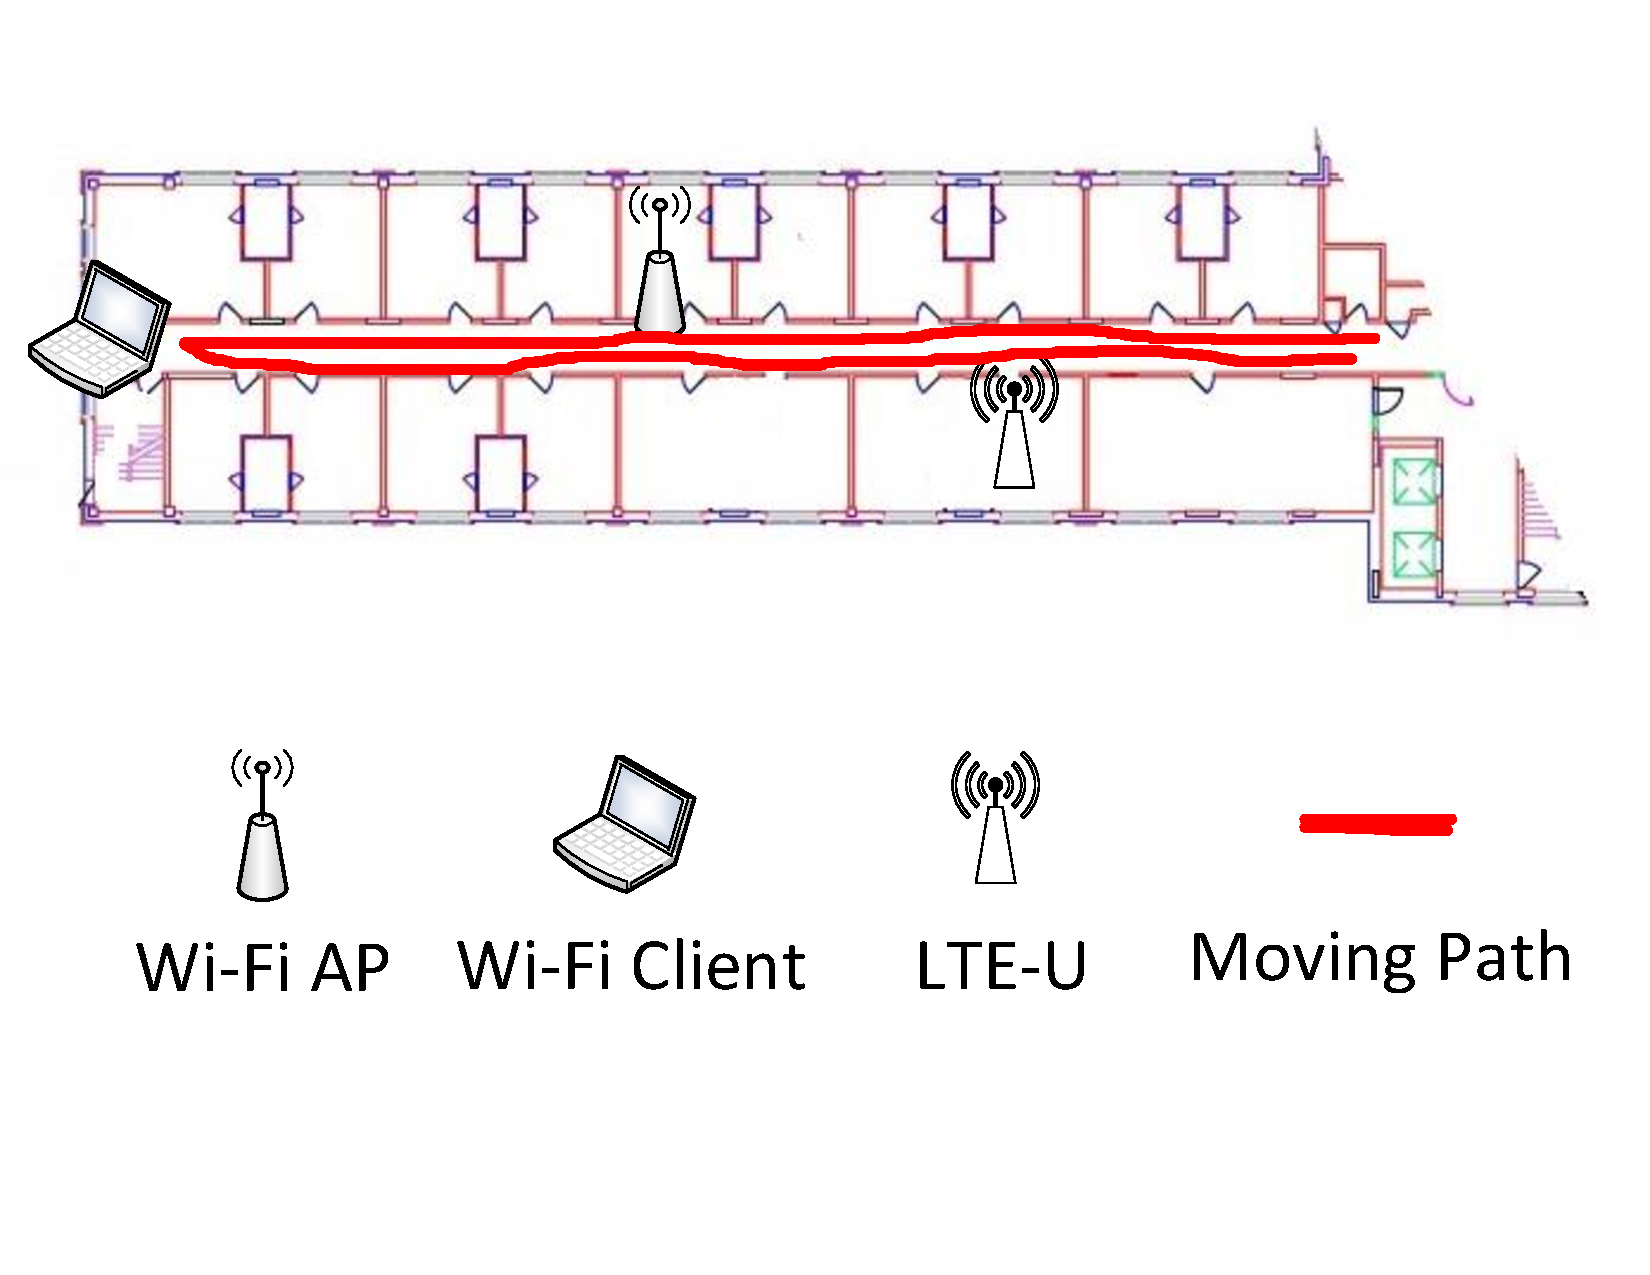
\includegraphics[width=0.26\textwidth]{./figures/floor_cs}
\hspace{-12pt}
    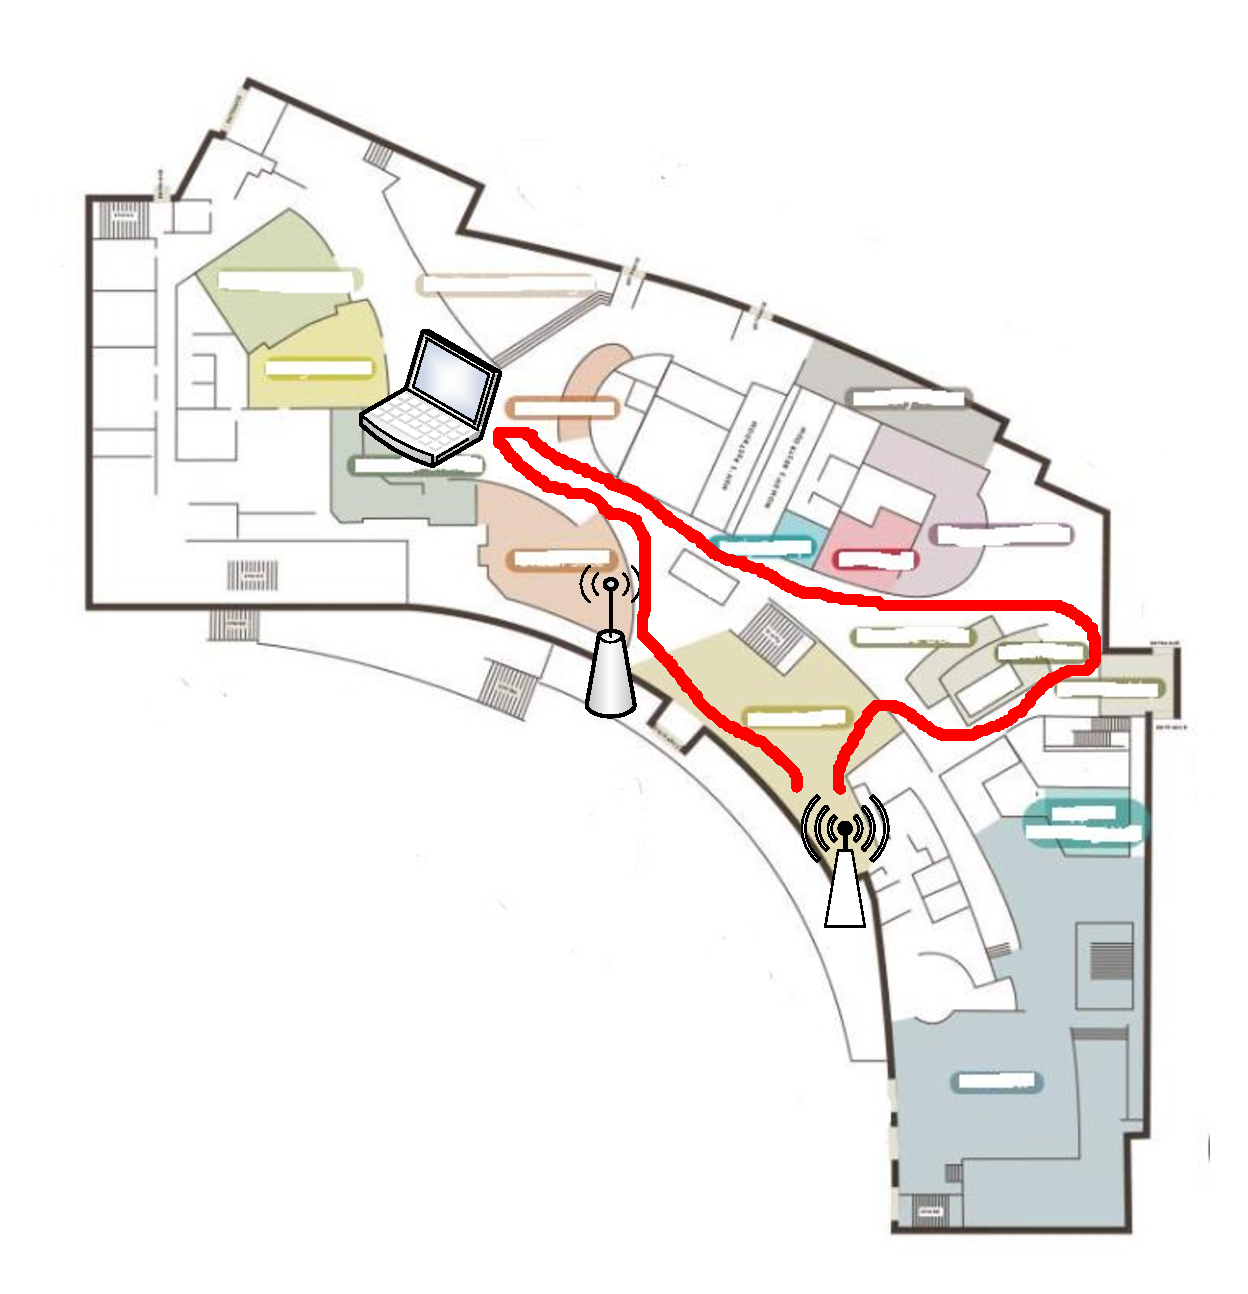
\includegraphics[width=0.23\textwidth]{./figures/floor_unionsouth}
\hspace{-24pt}
 \caption{Layout of the lab (left) and the cafeteria (right) with experiment locations.}
  \label{fig:wild_layout}
%\vspace{-12pt}
\end{figure}


In both cases we place the LTE-U node at one of the locations noted in Figure~\ref{fig:wild_layout}, and we move the measured Wi-Fi client around the coverage range of the measured Wi-Fi AP, following the trajectory denoted in Figure~\ref{fig:wild_layout} with a red line. We then move the LTE-U to the other location and repeat the measurements. 

In the first type of experiments we generated a saturated UDP downlink traffic from the measured AP to its client using iperf, and we record the achieved UDP rate and plot the CDF across all locations of the client and the AP. 
In the second type of experiments we download three web pages (www.google.com, www.youtube.com and www.facebook.com) and measure the total time required to download all three. 
We make a 1 second gap between the consecutive web request. 
The goal of this scenario is to illustrate how well different protocols adapt to a non-constant traffic. 
We record the completion times and plot the CDF across all locations of the client and the AP. 
The results are depicted in Figure~\ref{fig:wild_lab}. 
% and Figure~\ref{fig:wild_cafe}.

For each type of traffic we run five different experiments. 
First, we record the Wi-Fi traffic on the measured link without any added interference (red line, Solo).
Then, we record the Wi-Fi traffic on the measured link with added reference Wi-Fi AP (green line, Wi-Fi).
Finally, we record the Wi-Fi traffic on the measured link with added reference LTE-U AP, running CSAT with -62dBm threshold, 
CSAT with -82dBm threshold, and RAT with -82dBm threshold (blue, magenta and light blue lines, respectively).


\begin{figure*}[htb!]
 \centering
    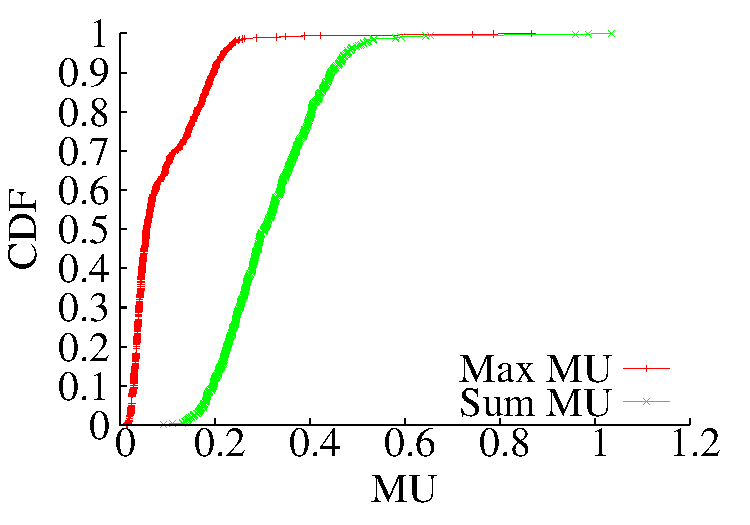
\includegraphics[width=0.31\textwidth]{./figures/mu-lab}
    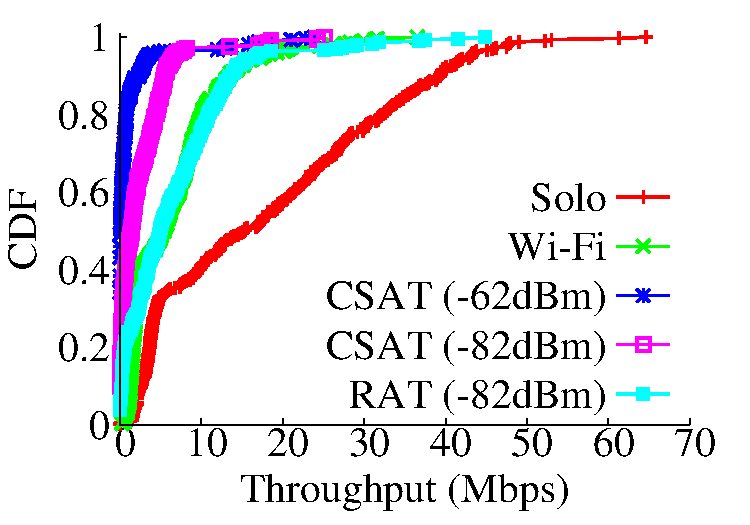
\includegraphics[width=0.31\textwidth]{./figures/office}
    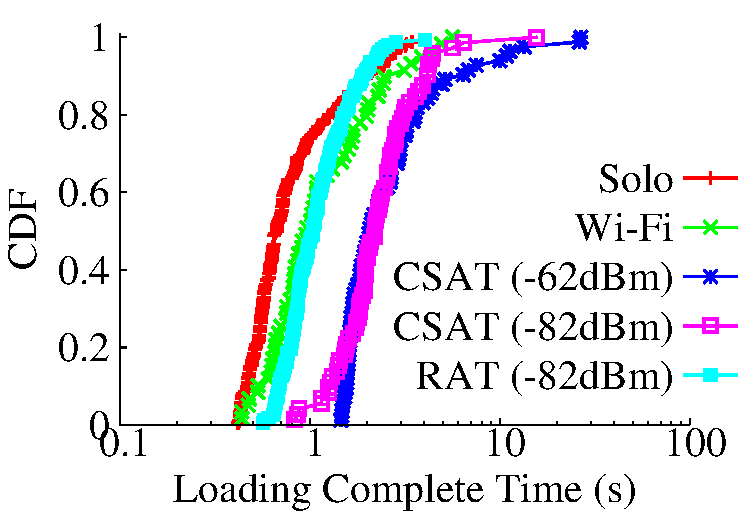
\includegraphics[width=0.31\textwidth]{./figures/officehttp}
    \vspace{-0.3cm}
 \caption{Lab: Estimated Wi-Fi utilization before the experiment (left), throughput of the measured Wi-Fi link for fully saturated UDP traffic (center) and for HTTP download (right).}
  \label{fig:wild_lab}
    \vspace{-0.3cm}
\end{figure*}

The results for the lab scenario are shown in Figure~\ref{fig:wild_lab}. 
Figure~\ref{fig:wild_lab}, center, we plot the CDF of the UDP rates for five different cases. 
As one can see, detection threshold of -62 dBm starves the measured Wi-Fi link in almost all the cases. 
Wi-Fi rate improves when we decrease the detection threshold to -82 dBm, but not substantially. 
This is because CSAT in many cases underestimated the medium utilization of the measured Wi-Fi link. 
Using a different adaptation mechanism RAT is able to substantially improves the performance of the Wi-Fi link, 10x in the median case. 
We also see that the throughput achieved by the measured Wi-Fi link is the same in presence of the other Wi-Fi node as it is in presence of an LTE-U node with RAT. 
%According to our definition of fairness (Section~\ref{sec:fairness}), this means that in this example LTE-U with RAT is fair to Wi-Fi. 

In Figure~\ref{fig:wild_lab}, right, we plot the CDF of the page download times. Here we see that the change in the energy detection threshold does not substantially improve the page download time. 
This is because the CSAT cannot track very well the change in the traffic and gets overly aggressive (similar to the Bilibili scenario, discussed in Section~\ref{sec:csat}). On the other hand RAT is able to achieve fairness with the measured Wi-Fi link. 
We also note that the RAT (blue) and Wi-Fi (green) lines do not coincide because we couldn't reproduce the exact same wireless environment although we walked a similar path. 
Nevertheless, the two figures are very similar.
We repeat the same measurement in the cafeteria scenario and 
the results are similar to the lab case. 
As a conclusion, we observe that CSAT almost always starved Wi-Fi networks and that RAT significantly improved coexistence. 

\nop{
\begin{figure*}[htb!]
 \centering
    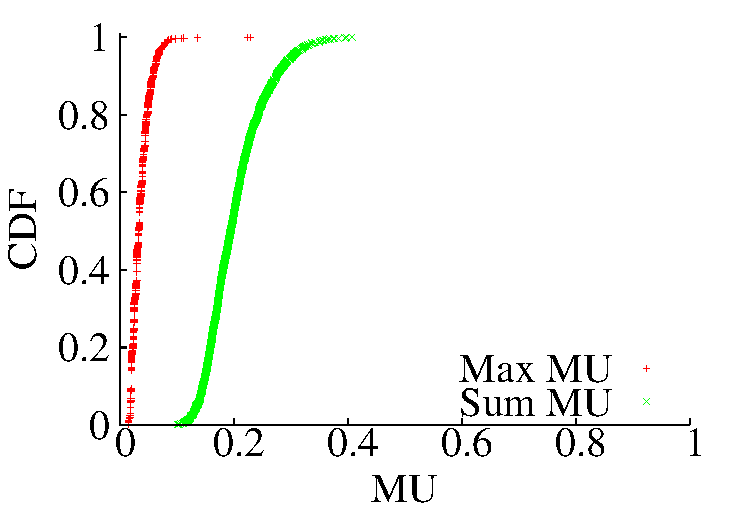
\includegraphics[width=0.31\textwidth]{./figures/union_mu}
    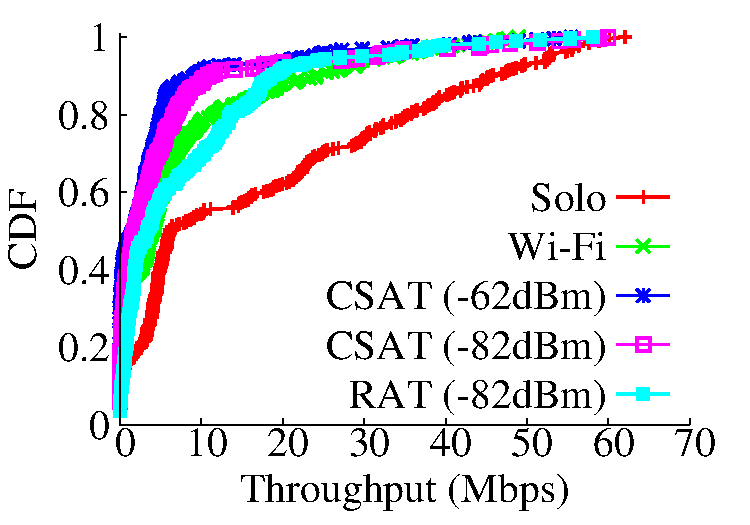
\includegraphics[width=0.31\textwidth]{./figures/unionsouth}
    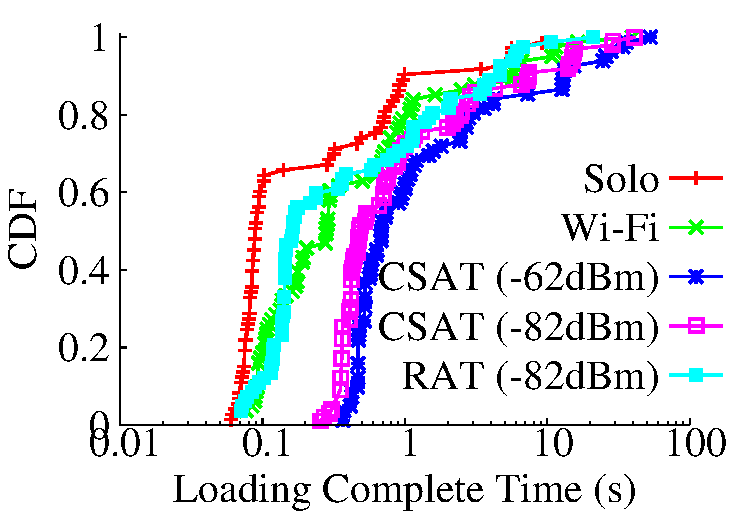
\includegraphics[width=0.31\textwidth]{./figures/httpunion}
 \caption{Cafeteria: Estimated Wi-Fi utilization before the experiment (left), throughput of the measured Wi-Fi link for fully saturated UDP traffic (center) and for HTTP download (right).}
  \label{fig:wild_cafe}
\end{figure*}
}

\nop{
In Figure~\ref{fig:wild_cafe}, we plot the same results for the cafeteria scenario. The conclusions are the same. LTE-U with CSAT highly affects the throughput of the measured Wi-Fi link and is not fair, regardless of the sensing threshold. In the same environment LTE-U with RAT allows the measured Wi-Fi to achieve much higher rate, comparable to the Wi-Fi case, and can be considered fair to Wi-Fi. 
As a conclusion, we observe that CSAT almost always starved Wi-Fi networks and that RAT significantly improved coexistence. 
}
%We also note that in all cases RAT is very close to Wi-Fi, and that we haven't observed much of the inefficiencies discussed in Section~\ref{sec:ineff}, because we used fully saturated LTE-U traffic in all our experiments. 



\nop{
Finally, we look at the effects of CTS-to-self in the real-world networks. We use TP Link AP for the measured AP since we have previously observed (Section~\ref{sec:rateadapt}) that its rate adaptation algorithm is affected by collisions. We run LTE-U with RAT and with and without CTS-to-self and we record UDP rates. The results are depicted in Figure~\ref{fig:ctself}. 

\begin{figure}[htb!]
\vspace{-12pt}
 \centering
    \includegraphics[width=0.35\textwidth]{./figures/cts}
\vspace{-12pt}
 \caption{CTS-to-self}
  \label{fig:ctself}
\end{figure}

We see that LTE-U with RAT and without CTS-to-self greatly affects the measured Wi-Fi link and almost halves its throughput. Once CTS-to-self is enabled, the Wi-Fi traffic is almost the same as in the reference Wi-Fi case. Again, we conclude that in this scenario LTE-U with RAT and CTS-to-self is fair to Wi-Fi. 
}
